\subsection{Vorbereitung der Daten und deskriptive Analysen}
Die erhobenen Daten wurden mittels SPSS Version 25 für Mac OS X aufbereitet. Die Stichprobendaten wurden direkt aus der Enterprise Feedback Suite \cite{Questback2018} mittels Datenexport für SPSS exportiert. Allfällige Fehlerquellen wurden bei der Datenbereinigung korrigiert. Dies wurde durch die Umfragesoftware erleichtert, indem nur abgeschlossene Datensätze exportiert wurden und eine erste Werteprüfung bereits bei der Eingabe erfolgte (z.B.: es wurden nur Zahlen bei der Eingabe des Jahrgangs zugelassen). Fehlende Werte wurden bereits von der Umfragesoftware gesetzt und konnten innerhalb von SPSS mit einem Wertelabel versehen werden. Für die Berechnung der Mediennutzung, der Bindung, des Stressniveaus und des subjektiven Wohlbefindens wurden zusätzliche Variablen in SPSS erstellt und anhand der generierten Daten berechnet (für die Formel der Berechnung siehe Kapitel \titleref{sec:Design}).

\subsubsection{Medien und Mediennutzung}

\begin{figure}
\centering
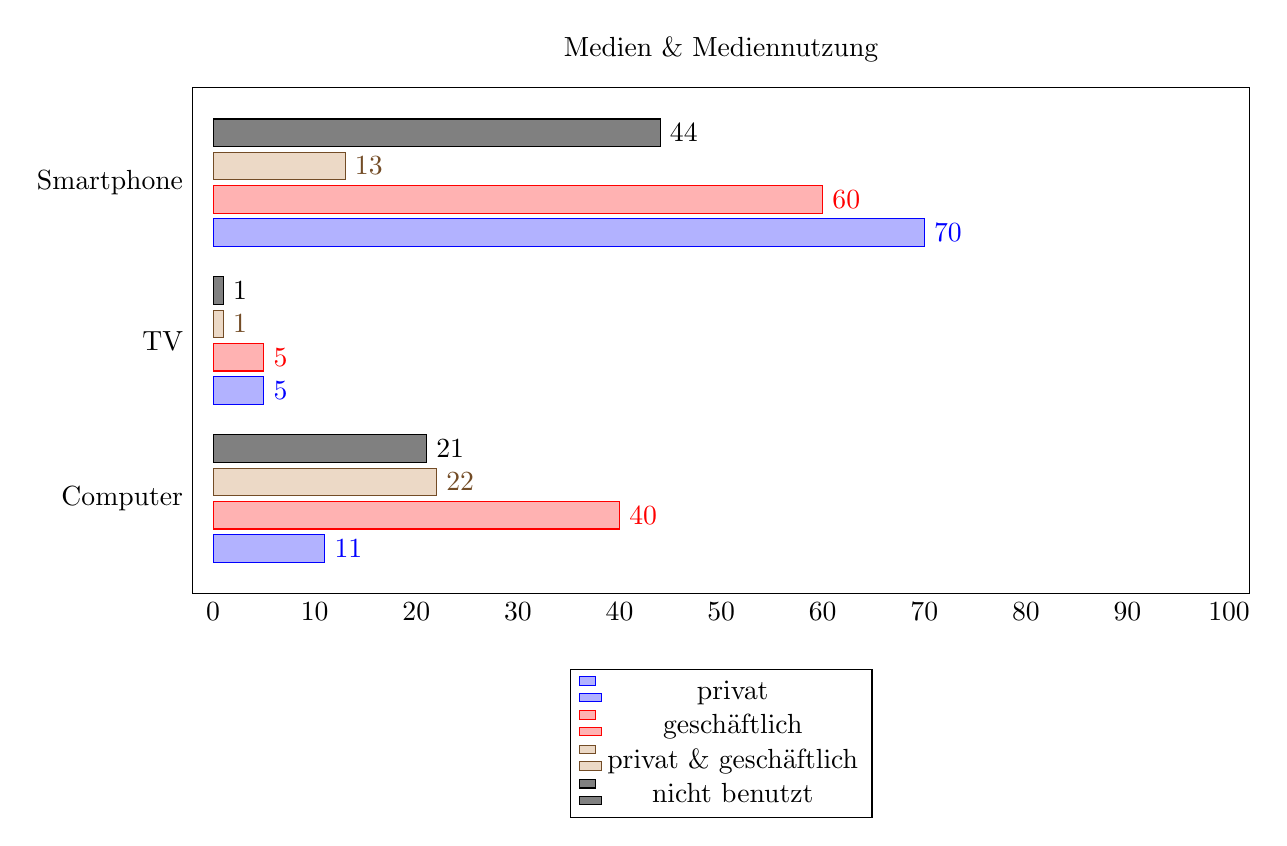
\begin{tikzpicture}[scale=1.0, auto,swap]
  \begin{axis}[title  = Medien \& Mediennutzung,
    xbar,
    %y axis line style = { opacity = 0 },
    %axis x line       = none,
    tickwidth         = 0pt,
    xmin              = 0,
    xmax              = 100,
    enlarge y limits  = 0.3,
    enlarge x limits  = 0.02,
    legend style={at={(0.5,-0.15)},
		anchor=north},
    ytick             = data,
    %ylabel            = Population,
    %xlabel            = {Mediennutzung},
    height            = 8cm,
    width             = 15cm,
    symbolic y coords = {Computer, TV, Smartphone},
    nodes near coords,
    nodes near coords align={horizontal},
  ]
  %privat
  \addplot coordinates { (70,Smartphone)(5,TV)(11,Computer)};
  %geschäftlich
  \addplot coordinates { (60,Smartphone)(5,TV)(40,Computer)};
  %privat und geschäftlich
  \addplot coordinates { (13,Smartphone)(1,TV)(22,Computer)};
  %nicht benutzt
  \addplot coordinates { (44,Smartphone)(1,TV)(21,Computer)};
  
  
  \legend{privat, geschäftlich, privat \& geschäftlich, nicht benutzt}
  \end{axis}
\end{tikzpicture}
\end{figure}

\subsubsection{Bindung anhand AAS}
\textit{TBD: Klassifizierung und Aufteilung in Sicher und Unsicher}.

% ---------------------------------------
\subsection{Hypothesentest} \label{sec:Hypothesentest}

% ---------------------------------------
\subsection{Zusätzliche Analysen} \label{sec:ZusätzlicheAnalysen}